\documentclass[../../main.tex]{subfiles}
\begin{document}

\subsection*{8.10}
Due conduttori cilindrici molto lunghi di raggio R, paralleli tra loro a notevole distanza l'uno dall'altro, sono percorsi dalle correnti $i_1$ e $i_2$ in versi opposti.\\
La circuitazione del campo magnetico lungo i percorsi chiusi $C_1$ e $C_2$ indicati in figura vale rispettivamente $\Gamma_1(B) = 0$ e $\Gamma_2(B) = -20\pi * 10^{-7}\ Tm$.\\
Calcolare $i_1$ e $i_2$.\\
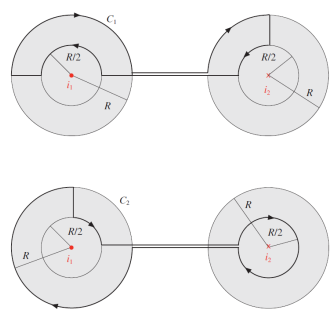
\includegraphics[scale=0.3]{e_8_10.png}
\subsubsection*{Formule utilizzate}
$\oint\vec{B}d\vec{s} = \mu_0\ i_{conc}$
\subsubsection*{Soluzione punto a}
Sappiamo che $C_1 = \oint\vec{B}d\vec{s} = 0$ e $C_2 = \oint\vec{B}d\vec{s} = -20\pi * 10^{-7}\ Tm$\\
$i_{conc} = i_A + i_B$\\
utilizzando una proporzione $i_A * \frac{1}{2}\pi\left(R^2-\frac{R^2}{4}\right) = i_1\pi R^2$ \\
$i_A = i_1* \frac{3}{8}$ e $i_B = \frac{3}{16}i_2$\\
$i_A$ avrà segno negativo, invece $i_B$ ha segno positivo\\
ottenitamo: $\Gamma_1(\vec{B}) = \mu_0\left(-i_A+i_B\right) = -\frac{3}{8}\mu_0\left(i_1-\frac{i_2}{2}\right) = 0$\\
Stesso procedimento per la seconda situazione:\\
$i_A = \frac{13}{16}i_1$ negativo.
$i_B = \frac{1}{4}i_2$ positivo.
La corrente è proporzionale alla superficie.
\subsubsection*{Soluzione punto b}
\newpage

\end{document}